\documentclass[a4paper, 11pt]{book}
\usepackage{/home/nicolas/Documents/Enseignement/Prepa/bpep/fichiers_utiles/preambule}
\usepackage{booktabs}

\newcommand{\dsNB}{11}
\makeatletter
\renewcommand{\@chapapp}{Kh\^olles MPSI2 -- semaine \dsNB}
\makeatother

% \toggletrue{corrige}  % décommenter pour passer en mode corrigé

\begin{document}

\chapter{Sujet 1\siCorrige{\!\!-- corrig\'e}}
\section{Question de cours}

Étude de la résonance d'itensité pour le cirtcuit RLC série en RSF~: établir et
tracer l'allure de $I(x)$ en introduisant le facteur de qualité et la pulsation
réduite $x$.

\resetQ
\section{Filtre de \textsc{Wien}}

\begin{minipage}{0.45\linewidth}
    On considère le circuit ci-contre avec $e(t) = E_m \cos(\omega t)$. On note
    $u(t) = U_m \cos(\omega t + \varphi)$ et on pose $H_m = U_m / E_m$ .
    \begin{enumerate}
        \item Déterminer les valeurs limites de $u(t)$ à basse et haute
            fréquences.
    \end{enumerate}
    Les courbes représentatives de $H_m (\omega)$ et $\varphi(\omega)$ sont
    fournies par les figures ci-dessous.
\end{minipage}
\hfill
\begin{minipage}{0.45\linewidth}
    \begin{center}
        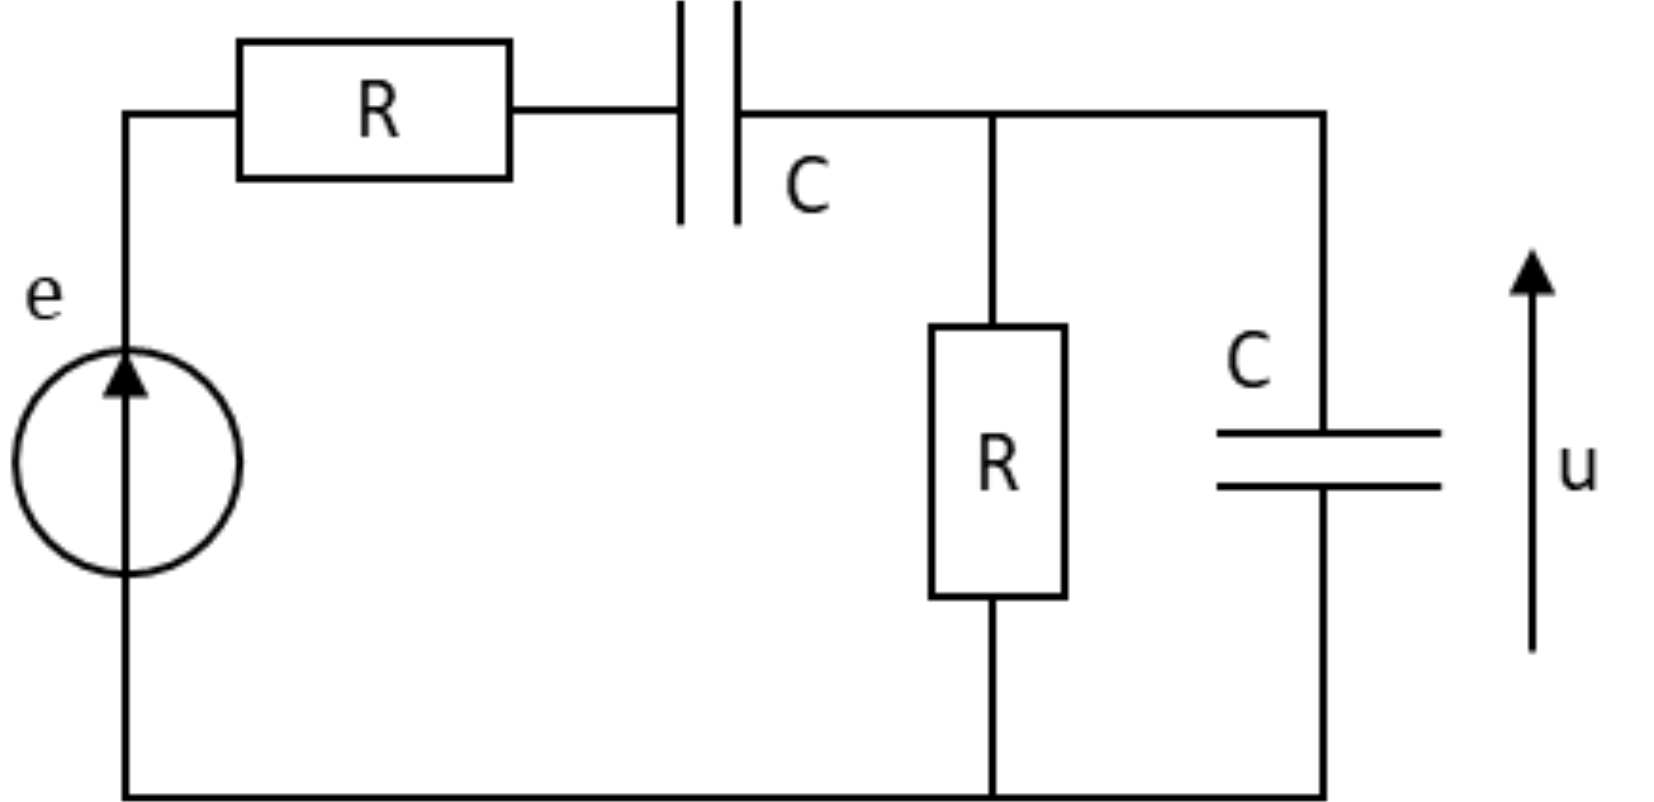
\includegraphics[width=\linewidth]{../../figures/ch11/wien_1}
    \end{center}
\end{minipage}

\begin{minipage}{0.45\linewidth}
    \begin{center}
        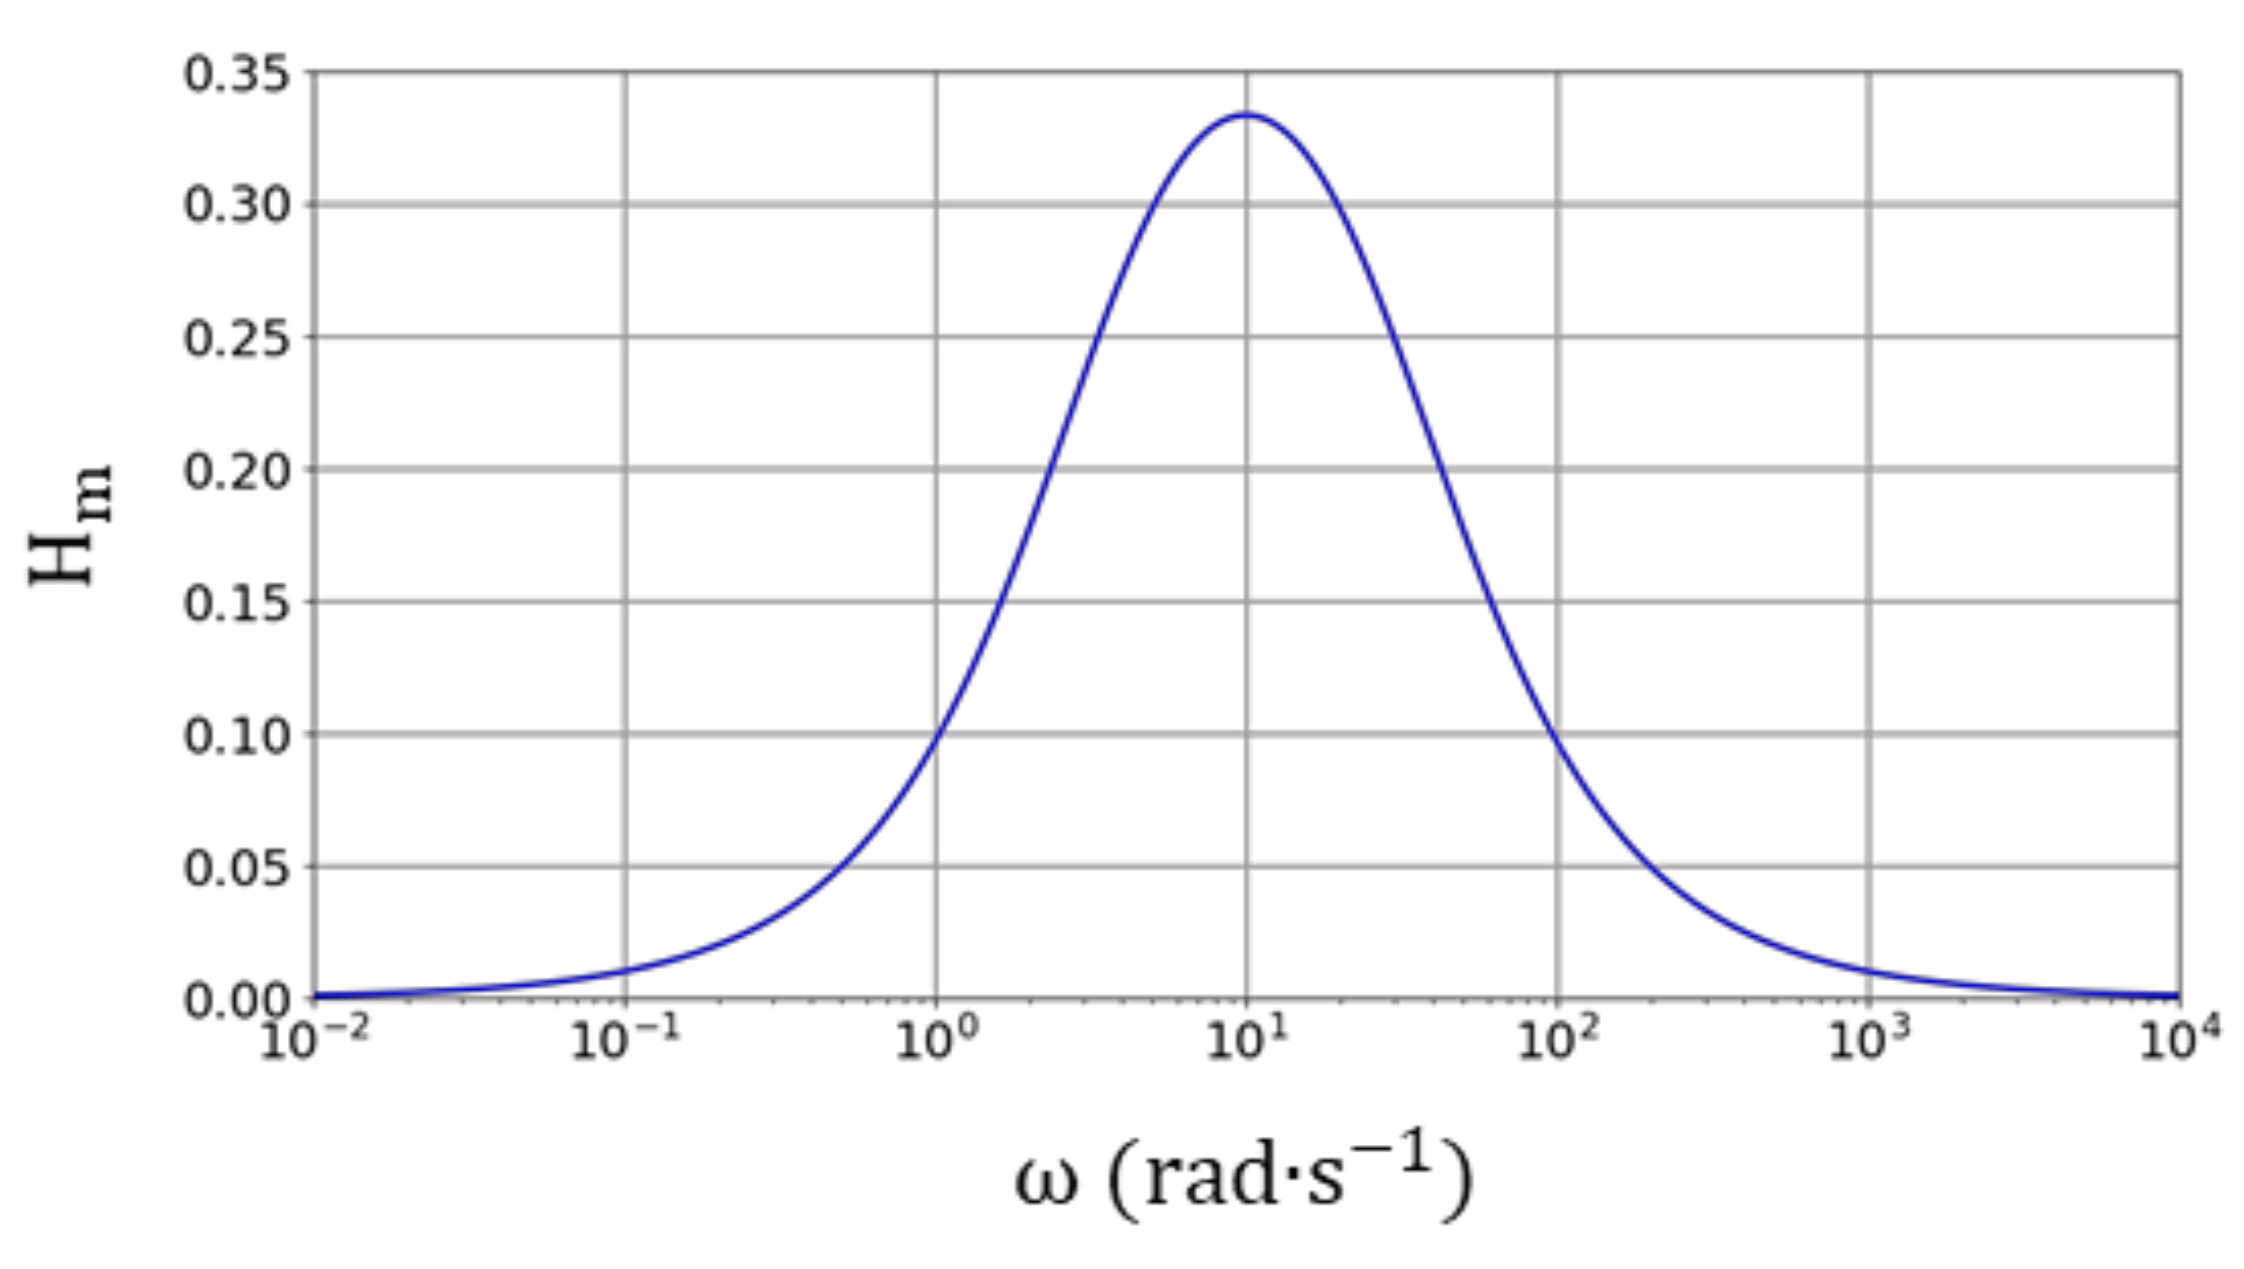
\includegraphics[width=\linewidth]{../../figures/ch11/wien_3}
    \end{center}
\end{minipage}
\hfill
\begin{minipage}{0.45\linewidth}
    \begin{center}
        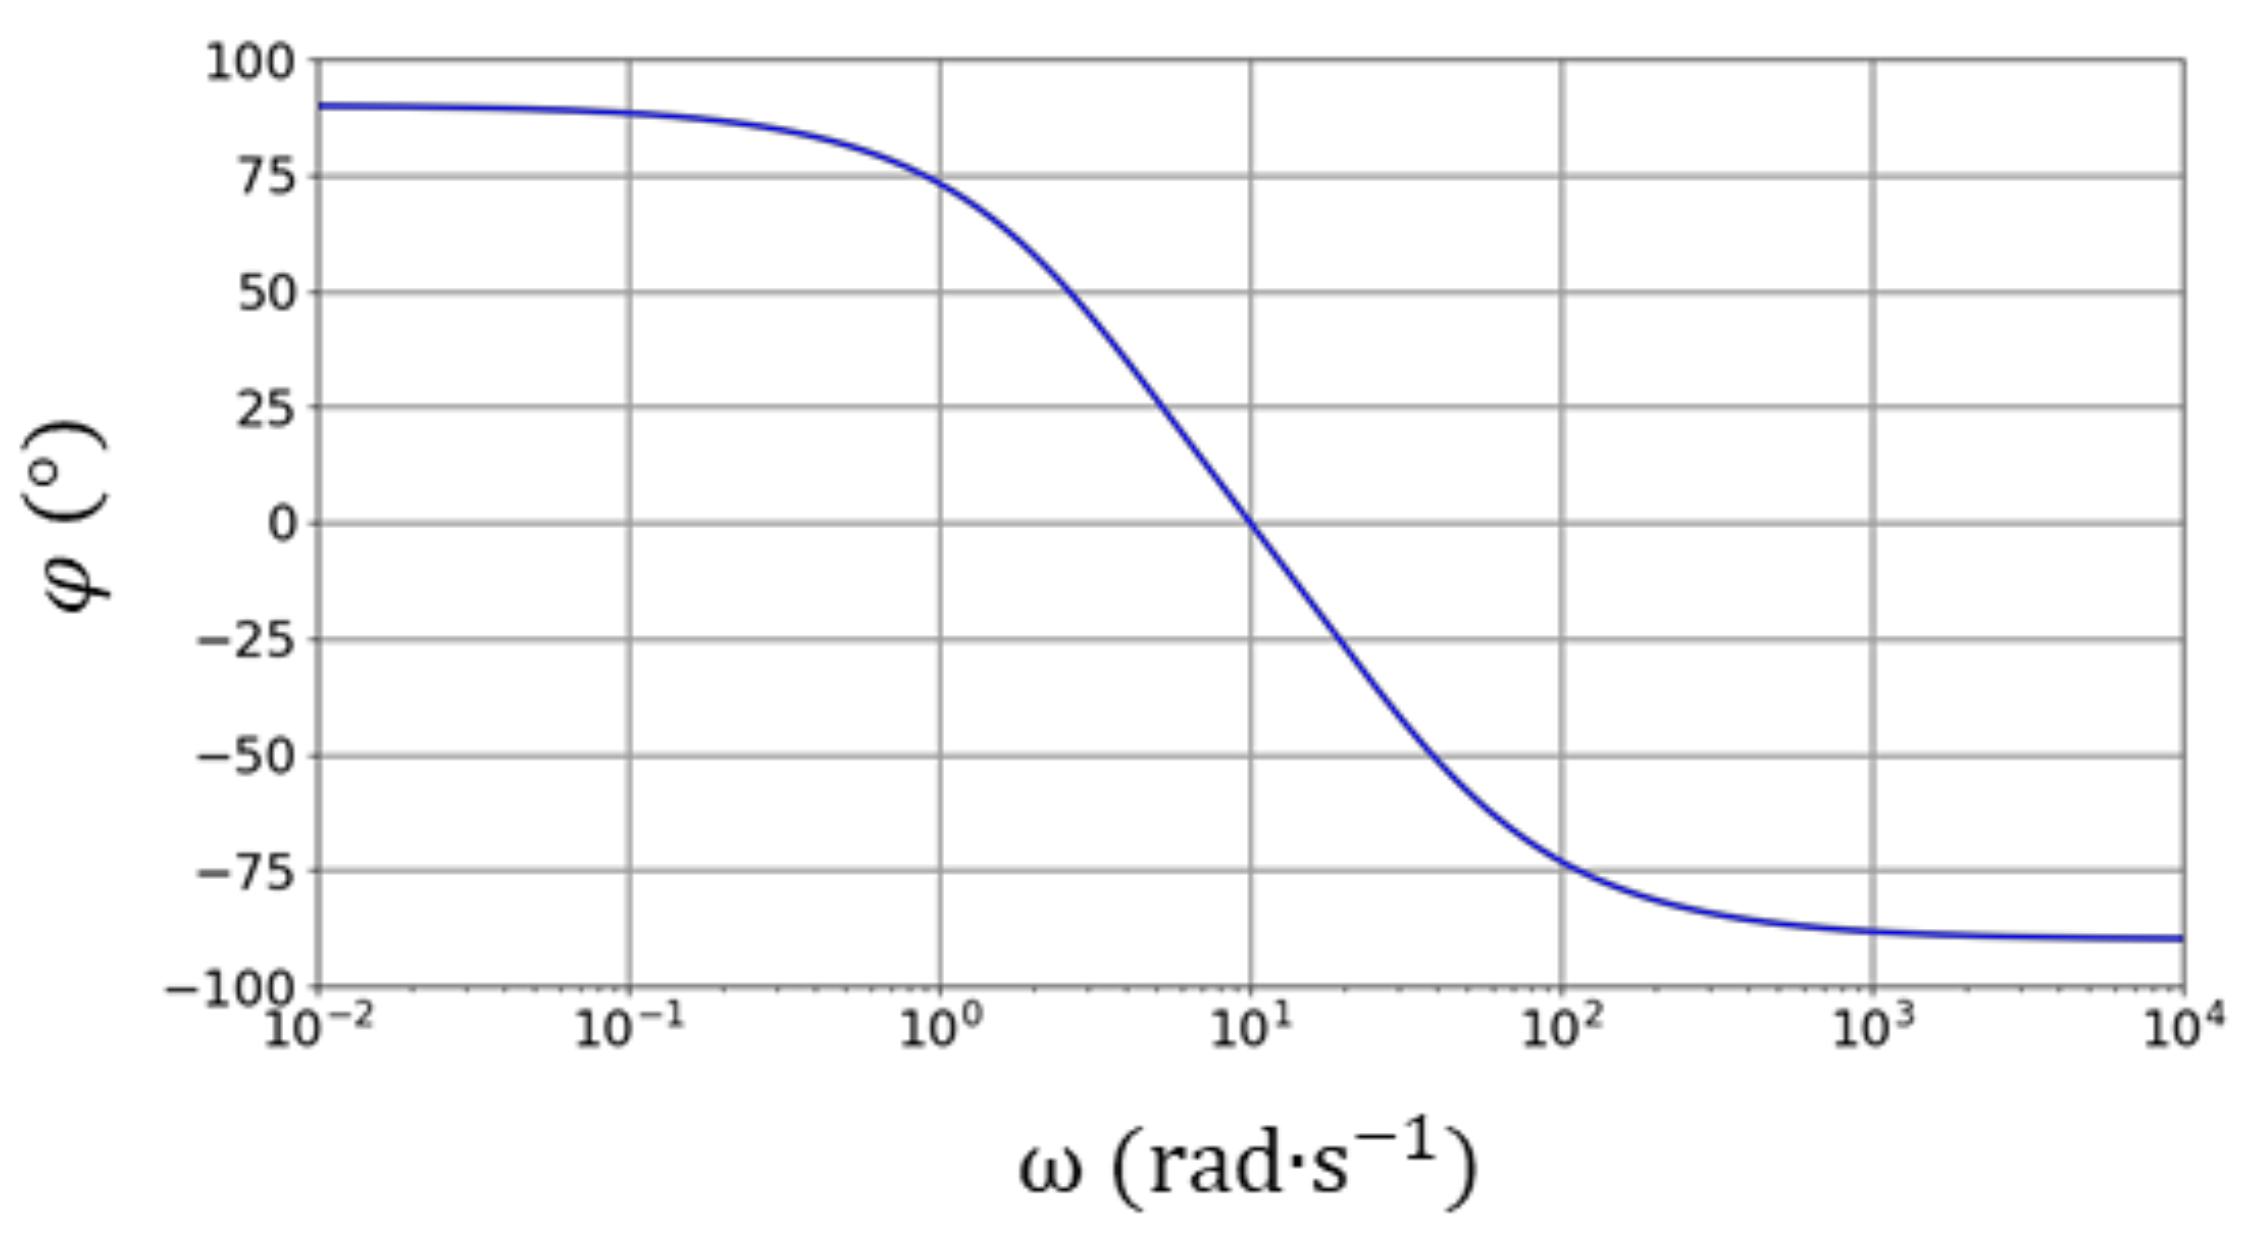
\includegraphics[width=\linewidth]{../../figures/ch11/wien_2}
    \end{center}
\end{minipage}

\begin{enumerate}[start=2]
    \item Observe-t-on un phénomène de résonance en tension~? Justifier.
    \item Déterminer graphiquement la pulsation de résonance, les pulsations de
        coupure et la bande passante du filtre.
    \item Après avoir associé certaines impédances entre elles, établir
        l'expression de $\ul{H} = \ul{u} / \ul{e}$. La
        mettre sous la forme~:
        \[
            \ul{H}
                = \dfrac{H_0}{1 + {\rm j} Q\left(x - \dfrac{1}{x}\right)}
            \qavec
            x = \dfrac{\omega}{\omega_0}
        \]
        avec $H_0$, $\omega_0$ et $Q$ des constantes à exprimer en fonction
        (éventuellement) de $R$ et $C$.
    \item Déterminer graphiquement la valeur du produit $RC$.
\end{enumerate}

\chapter{Sujet 2\siCorrige{\!\!-- corrig\'e}}
\section{Question de cours}

Lois d'associations des impédances en série et parralèle (énoncés et
démonstrations). Exemple~:
\begin{center}
    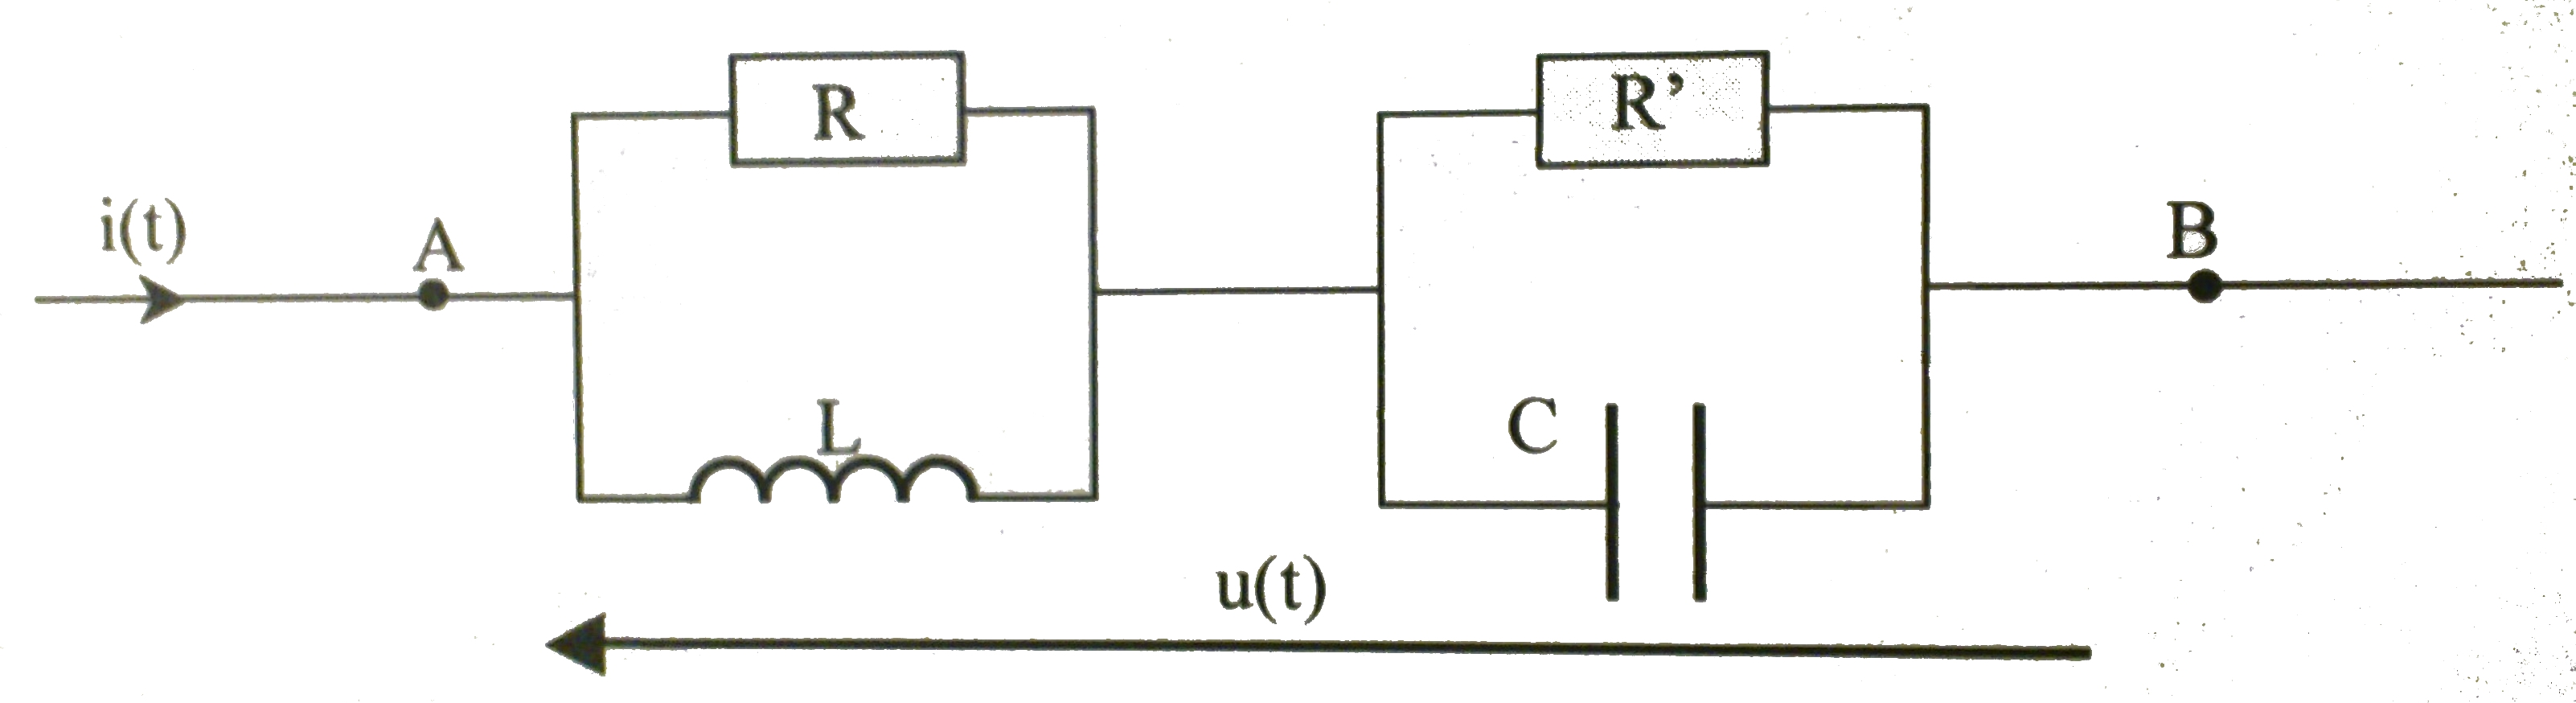
\includegraphics[width=.7\linewidth]{../../figures/ch11/circuit_2}
\end{center}

\resetQ
\subimport{/home/nicolas/Documents/Enseignement/Prepa/bpep/exercices/TD/vibration_moteur/}{sujet.tex}

\chapter{Sujet 3\siCorrige{\!\!-- corrig\'e}}
\section{Question de cours}

Étude de la résonance en élongation pour l'oscillateur mécanique horizontal en
RSF~: établir $X_u()$, $u$ étant la pulsation réduite, tracer l'allulre de
$X(u)$ et préciser la condition de résonance.

\resetQ
\section{Résonance d'un circuit bouchon}

\begin{minipage}{0.55\linewidth}
    
On considère le circuit $RLC$ représenté ci-contre, composé d'un
résistor, de résistance $R$, d'une bobine idéale d'inductance $L$,
d'un condensateur idéal, de capacité $C$, alimenté par une source
idéale de tension, de f.e.m. $e(t)=E_0\cos(\omega t)$. On se place en
régime sinusoïdal forcé.
\end{minipage}
\hfill
\begin{minipage}{0.45\linewidth}
    \begin{center}
        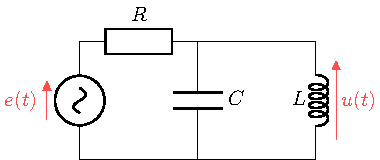
\includegraphics[width=\linewidth]{../../figures/ch11/bouchon_plain}
    \end{center}
\end{minipage}

\begin{enumerate}
    \item Exprimer l'amplitude complexe $\ul{U}$ de $u(t)$ en
        fonction de $E_0$, $R$, $L$, $C$ et $\omega$.
    \item Établir qu'il existe un phénomène de résonance pour la tension
        $u(t)$. Préciser la pulsation $\omega_0$ à laquelle ce phénomène se
        produit et la valeur de l'amplitude réelle de $u(t)$ à cette
        pulsation.
    \item Mettre l'amplitude réelle $U$ de $u(t)$ sous la forme: \[U =
            \dfrac{E_0}{\sqrt{1 + Q^2\left(\dfrac{\omega}{\omega_0} -
        \dfrac{\omega_0}{\omega}\right)^2}}\] avec $Q$ un facteur sans
        dimension à exprimer en fonction de $R,L$ et $C$.
    \item Exprimer la bande passante $\Delta\omega$ de cette résonance en
        fonction de $Q$ et $\omega_0$.
    \item En déduire les valeurs numériques de $C$ et $E_0$ à l'aide du
        graphe ci-dessous représentant l'amplitude réelle de $u(t)$ en
        fonction de la fréquence $f=\omega/2\pi$, sachant que $L= \SI{1}{mH}$ et
        $R= \SI{1}{k\Omega}$.
\end{enumerate}

\begin{center}
    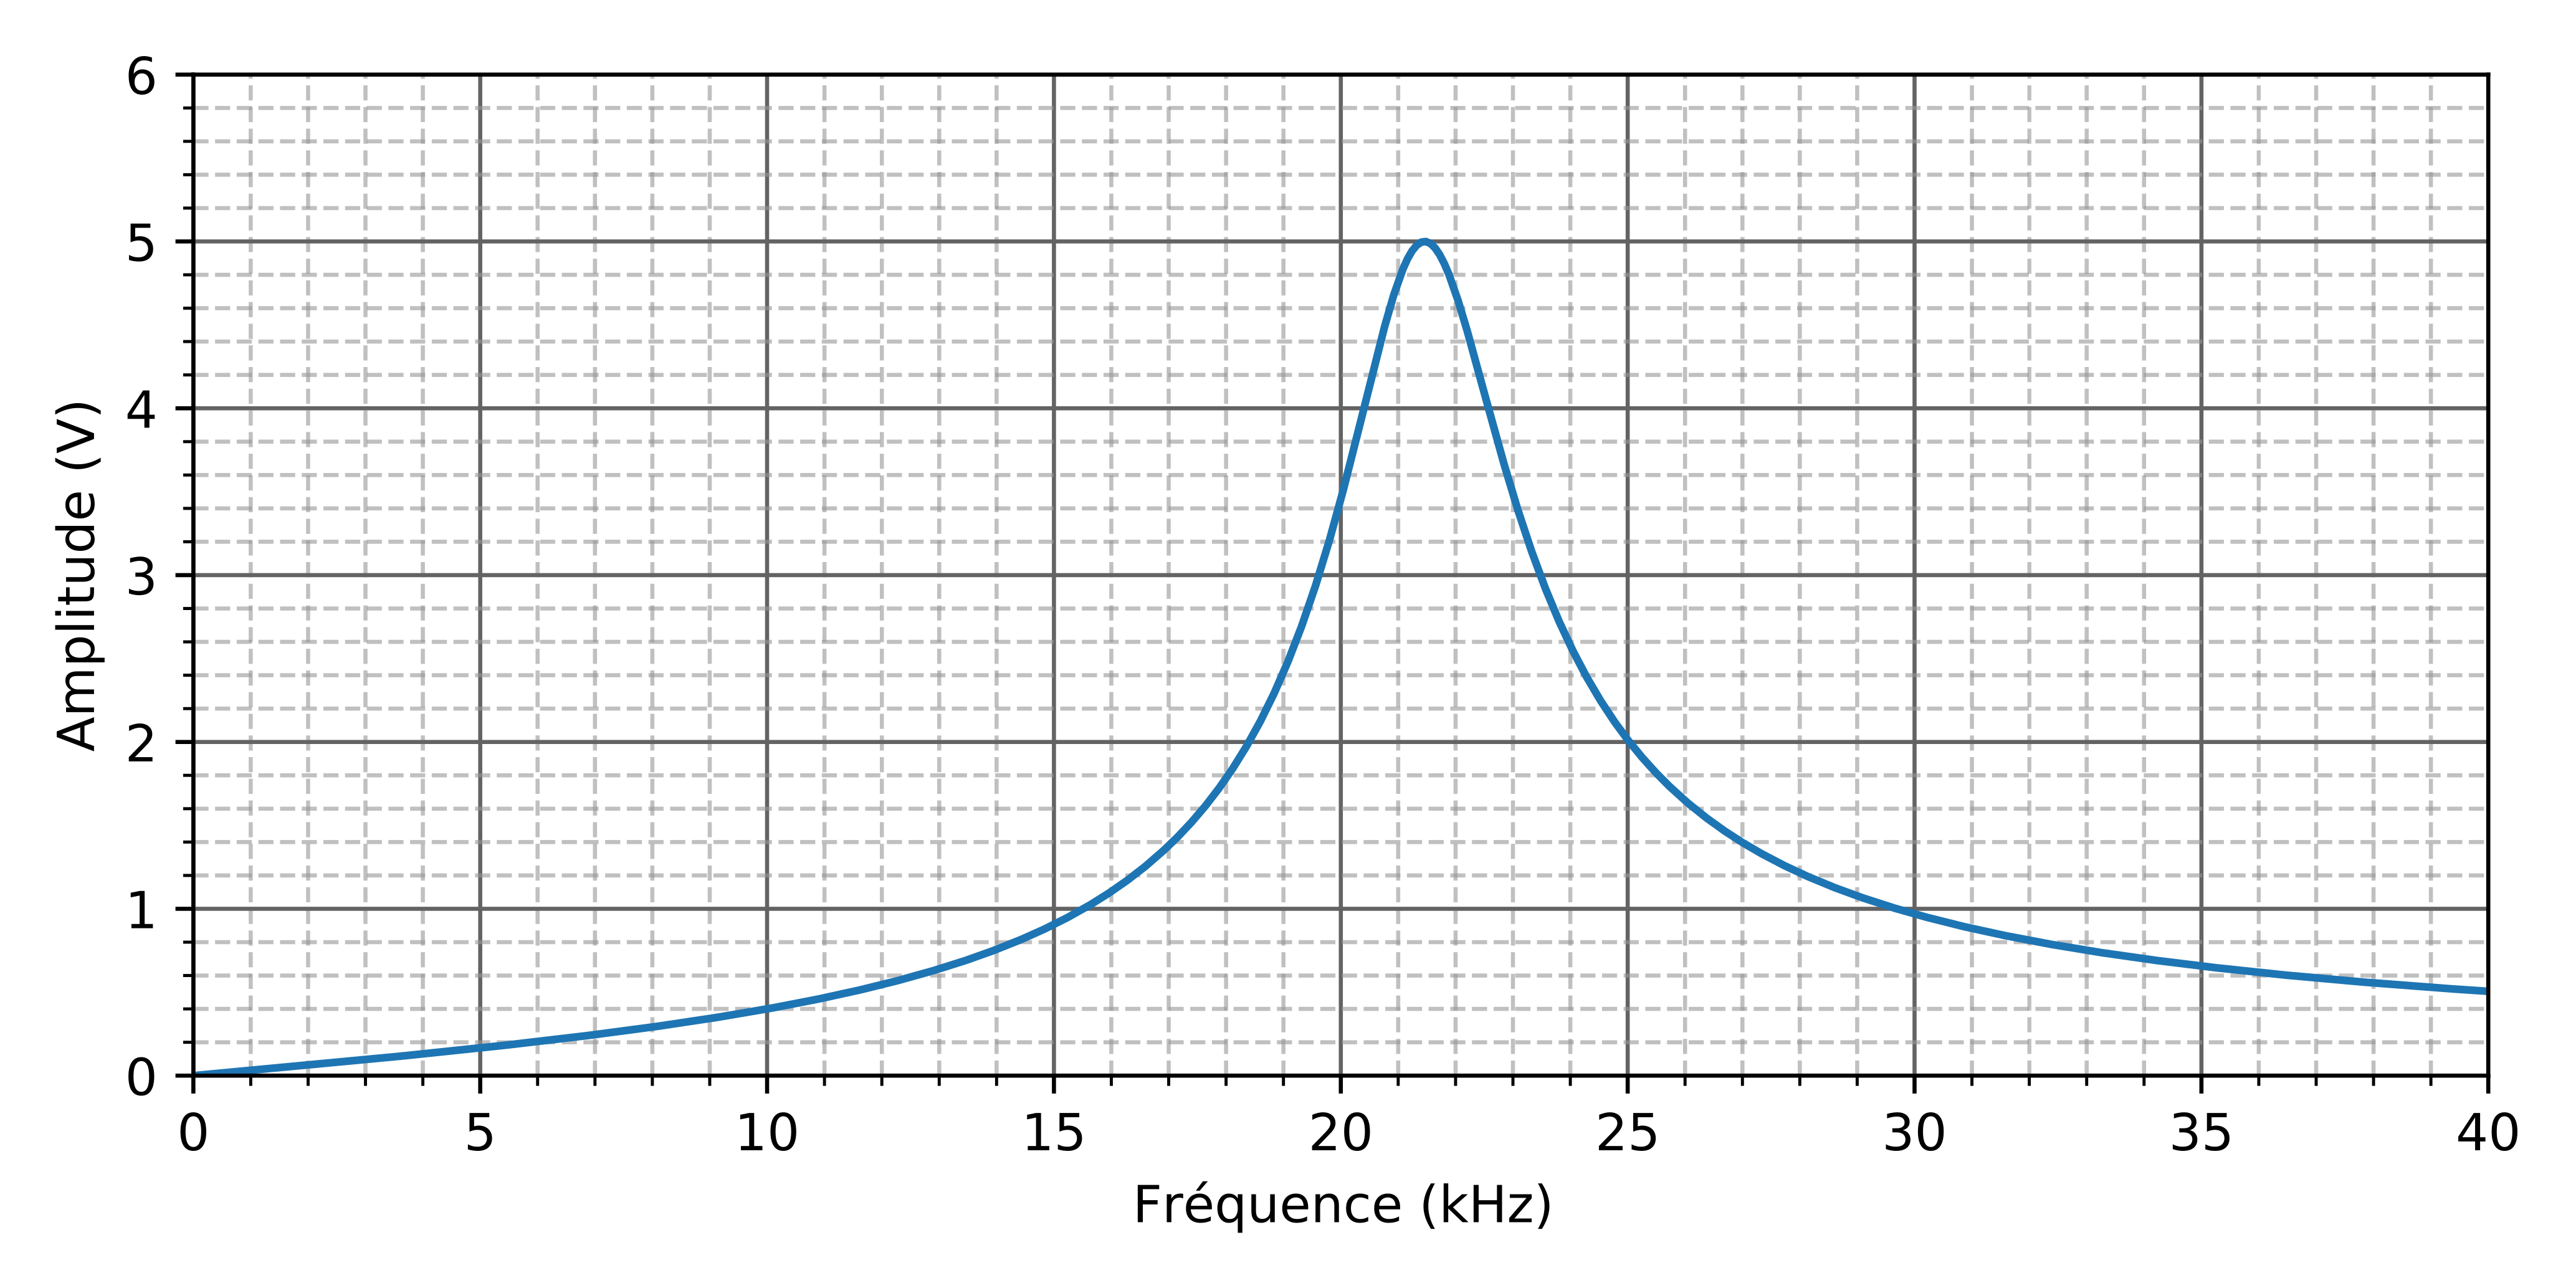
\includegraphics[width=.8\linewidth]{../../figures/ch11/bouchon_2}
\end{center}

\end{document}
